\chapter{Základní problematika virtualizace síťových funkcí}

Tato kapitola se zabývá základní analýzou a popisem problematiky spojené s oblastí virtuální síťových funkcí. Nejprve uveden přehled a krátký popis virtualizace a cloud computingu spolu s jejich přínosem pro IT. Následně je vysvětlena potřeba virtualizace síťových funkcí. Zde jsou porovnány jednotlivé přístupy k řešení a návrhu počítačových sítí. Zárověň je zde vysvětlen i základní koncept virtualizace síťových funkcí.

\section{Virtualizace a Cloud Computing}

Virtualizace je technologie, která změnila způsob, jakým se přistupuje k IT infrastruktuře. V tradičním modelu IT infrastuktury servery podporují pouze jeden operační systém v daném čase. Na tomto systému obvykle běží pouze jedna aplikace. Přestože by na tomto systému mohlo běžet více aplikací, tak je lepší držet aplikace odděleně na různých systech z důvodu minimalizace potencionálních bodů selhání. Pokud například nastane s aplikací problém, tak častým řešením je restartování systému. Pokud by na systému bylo více aplikací, znamenalo by to jejich vyřazení z provozu po dobu restartu, který může trvat velice dlouho. \cite{VM_book}

Z výše zmíněných důvodů došlo k velkému rozvoji a nasazování virtualizace. Virtualizací obecně označujeme techniky, které umožňují k dostupným hardwarovým zdrojům přistupovat jiným způsobem, než jakým fyzicky existují. Je tomu díky softwaru, který tento hardware abstrahuje a vytvoří tím virtuální prostředí. Virtualizované prostředí se dá snadněji přizpůsobit potřebám uživatelů, případně skrýt pro uživatele nepodstatné detaily (jako např. rozmístění hardwarových prostředků). Tím je tedy umožněno na jednom fyzickém serveru provozovat více od sebe oddělených virtuálních strojů, které mají každý svůj vlastní operačních systému s aplikacemi.

Software, který slouží pro virtualizaci, se nazývá hypervisor. Jak zmiňuje Popel a Goldberg v \cite{VM_architektura}, tak existují tyto dva základní typy hypervisorů:

\begin{itemize}
\item Typ 1 (Nativní - Bare-metal) - Tento hypervisor běží přímo na fyzickém hardwaru. Tím umožňuje provozovat více operačních systému na jednom fyzickém stroji. Příkladem takového hypervisoru je VMware ESXi, XEN a KVM.
\item Typ 2 (Hostovaný) - Na rozdíl od předchozího případu tento typ hypervisoru běží v prostředí operačního systému. Příkladem je například velice oblíbený Virtualbox či VMware Workstation.
\end{itemize}

Obrázek \ref{fig:virtualization} zobrazuje schématický popis obou typů hypervisorů a jejich rozdíl.

\begin{figure}[h]
\begin{centering}
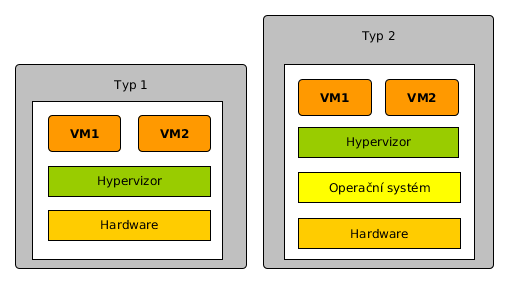
\includegraphics[scale=0.5]{images/virtualization}
\par\end{centering}
\caption{Schéma hypervisorů \label{fig:virtualization}}
\end{figure}

Virtualizace je základní technologie, na které je postavena virtualizace síťových funkcí. Ve většině připadů je však využití pouze jednoho hypervizoru telekomunikačními provozovately a velkými společnostmi nedostačující a je proto nutné využít cloud computingu.

Existuje několik definic pro cloud computing. Nejčastější používaná definice pro cloud computing je \cite{nist_definition}, kde je uvedeno, že je to  model umožnující využívání společného poolu počítačových zdrojů vzdáleně přes počítačovou síť. Tyto zdroje mohou být flexibilně alokovány a uvolňovány dle potřeby. Základní charakteristiky cloudu jsou tedy:

\begin{itemize}
\item Služby dostupné na požádání
\item Všudypřítomný přístup k síti
\item Sdílení zdrojů
\item Vysokou elasticitu
\item Měření využitých zdrojů
\end{itemize}

Z technického hlediska je cloud resp. cloudoví infrastruktura několik společně propojených serverů v clusteru. Na těchto serverech běží hypervisor, který vytvoří virtuální infrastrukturu. Tímto způsobem je tvořen společný pool zdrojů. Pro vytváření cloudových služeb zde ještě musí existovat cloudová platforma, která dokáže celou tuto virtuální infrastrukturu centrálně spravovat.

\section{Potřeba virtualizace síťových funkcí}


\section{Virtualizované síťové funkce - NFV}

//TODO Obrazek + popis jak je to dobry
//SW model

//TODO Obrazek pro Home
//TODO Obrazek pro Cloud
//TODO Obrazek pro Telco

Hlavní cíle tohoto řešení jsou zlepšit následující aspekty provozu telekomunikačních sítí:

\begin{itemize}
\item Smíření investičních nákladů – snížení potřeby nákupu jednoúčelových hardwarových zařízení, možnost platby pouze za využité kapacity a snížení rizik přílišného předimenzování kapacit
\item Snížení provozních nákladů – snížení prostoru, napájení a požadavky na chlazení, zjednodušení správy a řízení síťových služeb
\item Urychlení Time-to-market – zkrácení doby pro nasazení nových síťových služeb, chopení se nových příležitosti na trhu, vyhovění potřebám zákazníka
\item Doručit agilitu a flexibilitu – možnost rychle škálovat (rozšiřovat nebo zmenšovat služby) dle měnících se požadavků od zákazníka. Podpora služeb, které mají být dodány pomocí softwaru na libovolném standardním serverovém hardwaru
\end{itemize}

Jak je uvedeno v \cite{NFVState} a \cite{NFVChalanges}, tak celá myšlenka je založena na tom, že dojde k separování softwarové funkcionality v síťových prvcích od proprietárního hardwaru, na kterém běží. To umožní se síťovými funkcemi zacházek jako s klasickými softwarovými aplikacemi, které mohou běžet na standardním komerčně dostupných serverech jenž organizace v současnosti používají. Tím bude zároveň umožněno flexibilní nasazování těchto síťových funkcí a jejich dynamický provisioning. Díky tomu, že jsou síťová funkce odděleny od hardwaru, tak je také možné jejich vhodnější umístění v topologii. To znamená dle požadavků na umístění mohou být nasazeny v datových centrech, síťových uzlech či přímo v uživatelově koncovém bodě. Hlavní koncept virtualizace síťových funkcí znázorňuje obrázek č. \ref{fig:vize_NFV}. 

\begin{figure}[h]
\begin{centering}
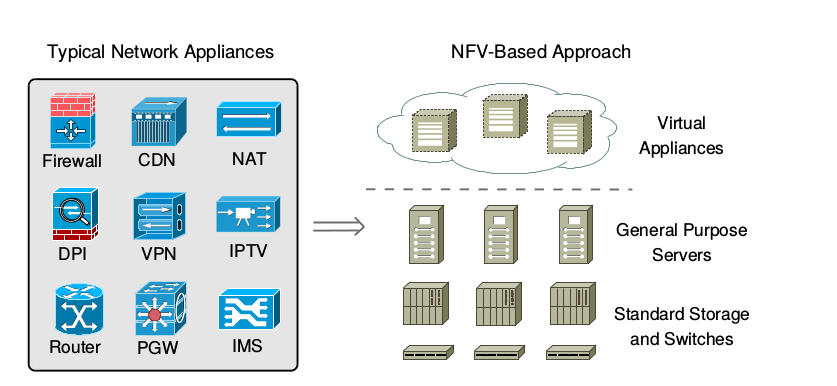
\includegraphics[scale=0.5]{images/vize_NFV}
\par\end{centering}
\caption{Koncept virtualizace síťových funkcí (NFV)\label{fig:vize_NFV}}
\end{figure}

Za zmínění stojí poznámka v \cite{NFVState}, kde je řečeno, že obecný koncept oddělení síťové funkce od hardwaru ještě nutně neznamená potřebu využití virtualizace. Protože budou síťové funkce dostupně jako software, tak mohou být nainstalovány a provozovány přímo na fyzickém stroji. Ovšem rozdíl je, že tento stroj již nebude speciální hardware, ale klasický server. Tento scénář může být do jisté míry použit při nasazovaní síťových funkcí v malém měřítku např. v uživatelských koncových bodech. Avšak pro plné využití všech výše zmíněných výhod, které jsou třeba ve velkých datových centrech, je třeba s použitím virtualizace počítat. To vše umocňuje fakt, že většina datových center v 

\section{NFV a softwarově definované sítě (SDN)}

Softwarově definované sítě (SDN) je jednou z dalších nových technologii, která se snaží vylepšit a automatizovat správu stávajících počítačových sítí. Dle \cite{SDN_clanek} jde o koncept, ve které je oddělena řídící logika (control plane) z jednotlivých routerů a switchů, které přeposílají traffic (data plane). Tím, že dojde k oddělení datové a řídící vrstvy, se routery a switche stanou pouze přeposílající data a veškerá řídí logika může být implementována v jednom logicky centrálním místě (SDN Controller). Z tohoto centrálního místa lze do jednotlivých routerů a switchů předávat instrukce pomocí aplikačních programovacích rozhraní (API). Samotný SDN Controller také obsahuje API, které mohou využívat aplikace a tím řídit, resp. programovat celou počítačovou síť.

\begin{figure}[h]
\begin{centering}
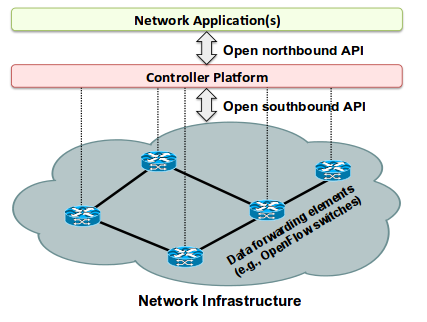
\includegraphics[scale=0.60]{images/SDN}
\par\end{centering}
\caption{Schéma SDN, převzato z \cite{SDN_clanek}\label{fig:SDN}}
\end{figure}

Obrázek č. \ref{fig:SDN} ukazuje jednoduché schéma softwarově definovaných sítí. Celou architekturu lze tedy rozdělit do 3 logických vrstev, které spolu komunikují pomocí API. 

\begin{itemize}
\item Aplikační vrstva - Na této úrovni se nachází samotné síťové aplikace jako jsou například DHCP, ACL, NAT, DNS a další. Jejich vytváření by
mělo být poskytováno prostřednictvím nižší vrstvy, nazývané northbound API.
\item Northbound APIs - Toto API využívají aplikace pro komunikaci s SDN controllerem. 
\item Control vrstva - V této vrstvě je centralizována veškerá logika, které dříve byla v síťových prvcích.
\item Southbound APIs - Jedná se o skupinu API protokolů, které pracují mezi vrstvou infrastruktury a control vrstvou. Jejím hlavním úkolem je komunikace, která povoluje SDN controleru instalovat na samotné síťové prvky rozhodnutí definované v aplikační vrstvě.
\item Vrstva infrastruktura - Nejnižší vrstvou je samotný hardware pro předávání datagramů na fyzické úrovni. Pro funkčnost celé architektury je nutné, aby zde byla nasazena zařízení, která umí přijímat pokyny od control plane skrze southbound API.

\end{itemize}

Přestože Softwarově definované sítě a virtualizace síťových funkcí jsou dvě různé technologie a koncepty, tak se navzájem se doplňují. Fakt, že SDN umožňuje programaticky ovládat počítačovou síť, lze využít pro poskytnutí programovatelné konektivity mezi jednotlivými virtuálními síťovými funkcemi. Naopak SDN může využít NFV tím, že implementuje potřebné síťové funkce jako software. Může tak virtualizovat SDN Controller, který tak může běžet na co nejvhodnějším místě v datovém centru. Je vidět, že tyto dvě technologie se dobře doplňují, proto jsou často součástí jednoho řešení. \cite{SDN_book}

\begin{figure}[h]
\begin{centering}
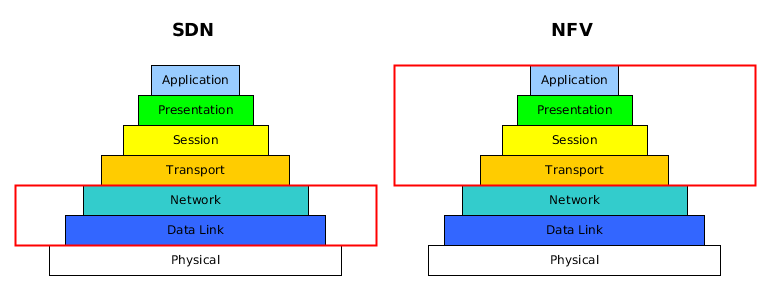
\includegraphics[scale=0.5]{images/sdn_nfv}
\par\end{centering}
\caption{ (NFV)\label{fig:vize_NFV}}
\end{figure}

//Tabulka rozdílů porovnani

\cite{Toward_NFV}

\subsection{Service Chaining} \label{sub:SDN}

Jednou z výhod NFV je možnost využít Service Chaining. Service chaining je ve skutečnosti součást SDN. Jde o princip jakým lze dynamicky pospojovat jednotlivé VNF a ovladat tak toky v síti. \cite{SDN_book}

Service chaining není ve skutečnosti nic nového. V klasických počítačových sítích je používán také, ale pomocí fyzických síťových prvků. Jedná se zjednodušeně o způsob zapojení mezi jednotlivými síťovými prvky (či VNF) a způsob, jakým na sebe navazují. Příklad takového zapojení je vidět na obrázku č. \ref{fig:service_chaining}. Zde se provozovatel sítě rozhodl, že odchozí data z klientských stanic musí jít přes firewall, IDS a nakonec přes NAT do Internetu. Příchozí data mají logicky obrácené pořadí. Toto zapojení funguje dobře pro síť, kde není třeba rozlišovat cestu jakou proudí data jednotlivých uživatelských stanic. Ale není to optimální řešení pro sítě s více uživateli, kde každý požaduje jinou síťovou funkci. Potřeba jednotlivých síťových služeb se samozřejmě může v čase měnit. Příklad takové sítě lze nalézt ve většině datových center. 

\begin{figure}[h]
\begin{centering}
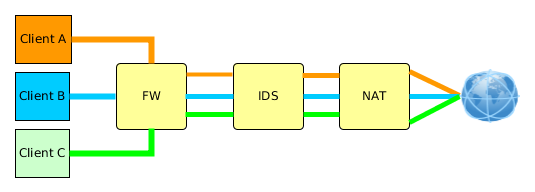
\includegraphics[scale=0.55]{images/service_chaining}
\par\end{centering}
\caption{Ukázka klasického service chainigu pomocí fyzických síťových prvků\label{fig:service_chaining}}
\end{figure}

Zde tedy přichází na řadu VNF spolu s SDN. Protože jednotlivé VNF existují jako virtuální stroje, tak mohou být dynamicky nasazovány dle aktuálním požadavků jednotlivých klientů a pomocí SDN mohou být tyto VM dynamicky pospojovány. Obrázek č. \ref{fig:service_chaining_new} ukazuje schéma zapojení, kde každý klient může mít jinou požadovanou cestu do internetu. Je možná i varianta, kde každý klient má své vlastní VNF s jinou konfigurací.

\begin{figure}[h]
\begin{centering}
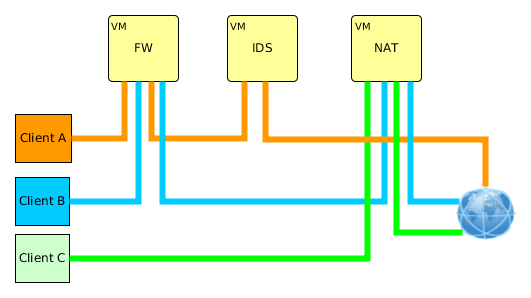
\includegraphics[scale=0.55]{images/service_chaining_new}
\par\end{centering}
\caption{Ukázka VNF service chainigu\label{fig:service_chaining_new}}
\end{figure}